
\section{Codebasis Umstrukturierung}

Wir haben uns dann als Team dazu entschlossen, dass die eigene Implementierung gescheitert war und etwas anderes versucht werden musste.
Die Idee war es, die vorhandene Implementierung zu nutzen, aber da der Code sehr schwer zu verstehen war und auch die Zeit so langsam ein 
Problem wurde, nur noch die Slices auf einem Cluster zu parallelisieren. Das Vorgehen dabei war es, den vorhandenen Code nicht wirklich zu 
verändern sondern, nur die vorhandenen Funktionen wieder zu verwenden. 
\newline 
\newline 
Der originale Code hatte eine Klasse \emph{LocalSubspaceTable}, die für das Darstellen der \emph{Subspace}-Tabelle zuständig war.
Diese Klasse wurde sowohl für die \emph{Slices} als auch für die gesamten \emph{Subspaces} verwendet. Meine Idee war es dann,
den anderen im Team eine Funktion names \emph{calculateRemote} bereitzustellen, die als Parameter die \emph{Labels}, den \emph{minBound} des Slices und den 
\emph{maxBound} des Slices bekommt und den berechneten Slice als Form der \emph{LocalSubspaceTable}-Klasse zurückgibt. 
\newline
\newline
Im Folgenden wird zunächst der Aufbau des originalen Code erläutert, um anschließend die Umsetzung der \emph{calculateRemote}-Methode
von unten nach oben darzustellen. 

\subsection{Aufbau des originalem Code}
Der Code bestand im wesentlichen aus einer abstrakten Klasse \emph{ISubscale} und zwei konkreten Implementierungen
\emph{Subscale} (\emph{Cuda}-Implementation) und \emph{SubscaleSec} (normale Implementation) wie im folgenden gezeigt:
\newpage
\begin{figure}[h]
    \centering
    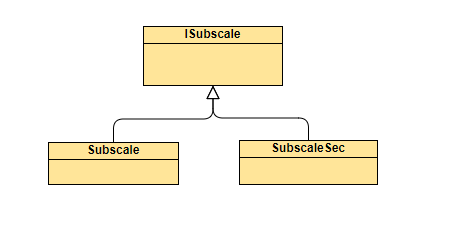
\includegraphics[width=\textwidth]{Subscale.png}
    \caption{Subscale}
    \label{img:subscale}
\end{figure}

\emph{ISubscale} selber hatte eine Funktion \emph{calculateClusterCandidates} die Vorbereitungen getroffen hat und die 
konkrete Implementierung sollte die Funktion \emph{calculateAllSlices} überschreiben, die den Zweck hatte, alle \emph{Slices}
zu erstellen und auf die Festplatte zu schreiben. Außerdem verfügte \emph{ISubscale} noch über eine Funktion \emph{combineAllSlices}
die die einzelnen Slices von der Festplatte geholt hat, die Slice verengert hat und dann zu der endgültigen Subspace Tabelle 
hinzugefügt hat.   

\subsection{calculateSlice}
Angefangen am untersten Ende brauchten die beiden konkreten Implementationen eine neue Funktion, die alle nötigen Informationen 
bekommt, um einen Slice zu erstellen und als Rückgabe dann den Slice zurückgibt. Da sich die konkreten Implementationen nur in der 
Erzeugung der konkreten Klassen unterscheidet, wird in dieser Section der generelle Code gezeigt und in den folgenden Abschnitten 
nur die wesentlichen Unterschiede.  

\lstinputlisting[language=C++,caption={calculateSlice},
    label=lst:calculateSlice]{src/calculateSlice.cpp}

Wie in Listing \ref{lst:calculateSlice} zu sehen ist, werden die Berechungsklassen initialisiert und anschließend werden die 
\emph{DenseUnits} erzeugt, um diese dann in eine Subspace Tabelle hinzuzufügen. Sollte der \emph{Slice} nicht leer sein, dann 
werden die Einträge noch nach den Subspaces zusammengefügt. Als letztes wird noch der Speicher von der Grafikkarte zum Host kopiert 
(ist bei der sequentiellen Abarbeitung nicht nötig). 

\subsection{calculateSlice Sequentiell}
In dieser Sektion werden noch die spezifischen Erzeugungen der Berechungsklassen für die Sequentielle Abarbeitung gezeigt.

\lstinputlisting[language=C++,caption={calculateSlice Sequentiell},
    label=lst:calculateSliceSeq]{src/calculateSliceSeq.cpp}

\subsection{calculateSlice Sequentiell}
In dieser Sektion werden noch die spezifischen Erzeugungen der Berechungsklassen für die \emph{Cuda} Abarbeitung gezeigt.

\lstinputlisting[language=C++,caption={calculateSlice Cuda},
    label=lst:calculateSliceCuda]{src/calculateSliceCuda.cpp}

\subsection{calculateClusterCandidatesRemote}
Die nächst obere Stufe war die \emph{calculateClusterCandidatesRemote}-Methode, die alle notwendigen 
Informationen für die \emph{calculateSlice} vorbereitet. Diese sieht wie folgt aus:

\lstinputlisting[language=C++,caption={calculateClusterCandidatesRemote},
    label=lst:calculateClusterCandidatesRemote]{src/calculateClusterCandidatesRemote.cpp}

Diese hat die \emph{CoreSets} erzeugt und die weiteren Informationen weiter runter gegeben.

\subsection{calculateRemote}
Der letzte Schritt war dann, die \emph{calculateRemote}-Methode, die lediglich die \emph{config}
gelesen hat und dann die konkrete Implementierung des \emph{Subscales} erzeugt hat. 

\lstinputlisting[language=C++,caption={calculateRemote},
    label=lst:calculateRemote]{src/calculateRemote.cpp}